% !TEX TS-program = pdflatex
% !TEX encoding = UTF-8 Unicode

\documentclass[a4paper, titlepage=false, parskip=full-, 10pt]{scrartcl}

\usepackage[utf8]{inputenc}
\usepackage[T1]{fontenc}
\usepackage[english, ngerman]{babel}
\usepackage{babelbib}
\usepackage{hyperref}
\usepackage{listings}
\usepackage{framed}
\usepackage{color}
\usepackage{graphicx}
\usepackage[normalem]{ulem}
\usepackage{cancel}
\usepackage{amsmath}
\usepackage{amssymb}
\usepackage{amsthm}
\usepackage{algorithm}
\usepackage{algorithmic}
\usepackage{geometry}
\usepackage{subfigure}
\geometry{a4paper, top=20mm, left=35mm, right=25mm, bottom=40mm}

\newcounter{tasknbr}
\setcounter{tasknbr}{1}
\newenvironment{task}[1]{{\bf Aufgabe \arabic {tasknbr}\stepcounter{tasknbr}} (#1):\begin{enumerate}}{\end{enumerate}}
\newcommand{\subtask}[1]{\item[#1)]}

% Listings -----------------------------------------------------------------------------
\definecolor{red}{rgb}{.8,.1,.2}
\definecolor{blue}{rgb}{.2,.3,.7}
\definecolor{lightyellow}{rgb}{1.,1.,.97}
\definecolor{gray}{rgb}{.7,.7,.7}
\definecolor{darkgreen}{rgb}{0,.5,.1}
\definecolor{darkyellow}{rgb}{1.,.7,.3}
\lstloadlanguages{C++,[Objective]C,Java}
\lstset{
escapeinside={§§}{§§},
basicstyle=\ttfamily\footnotesize\mdseries,
columns=fullflexible,
keywordstyle=\bfseries\color{blue},
commentstyle=\color{darkgreen},      
stringstyle=\color{red},
numbers=left,
numberstyle=\ttfamily\scriptsize\color{gray},
breaklines=true,
showstringspaces=false,
tabsize=4,
captionpos=b,
float=htb,
frame=tb,
frameshape={RYR}{y}{y}{RYR},
rulecolor=\color{black},
xleftmargin=15pt,
xrightmargin=4pt,
aboveskip=\bigskipamount,
belowskip=\bigskipamount,
backgroundcolor=\color{lightyellow},
extendedchars=true,
belowcaptionskip=15pt}

%% Enter current values here: %%
\newcommand{\lecture}{Robotik WS15/16}
\newcommand{\tutor}{}
\newcommand{\assignmentnbr}{4}
\newcommand{\students}{Julius Auer}
%%-------------------------------------%%

\begin{document}  
{\small \textsl{\lecture \hfill \tutor}}
\hrule
\begin{center}
\textbf{Übungsblatt \assignmentnbr}\\
[\bigskipamount]
{\small \students}
\end{center}
\hrule

\begin{task}{ROS-Services}
\item[]
\emph{srv\_set\_pose.cpp} implementiert den gewünschten Service und wird via launch-file gemeinsam mit dem bestehenden arm2r-Code gestartet. \emph{client.cpp} wird via \emph{rosrun} gestartet und erwartet als Argument einen Befehl, in welche Richtung der Arm bewegt werden soll. Es war nicht gefordert die \emph{.srv} mit einzureichen (hier: \emph{SetPose.srv}), welche aber auch denkbar uninteressant ist. Die eigentliche Schwierigkeit war hier, \emph{CMake} und \emph{launch} in den Griff zu bekommen.

Anbei Screenshots (Abbildung \ref{fig:1}) und Code:
\begin{figure}[!htpb]
\centering
\subfigure[nach links]{
  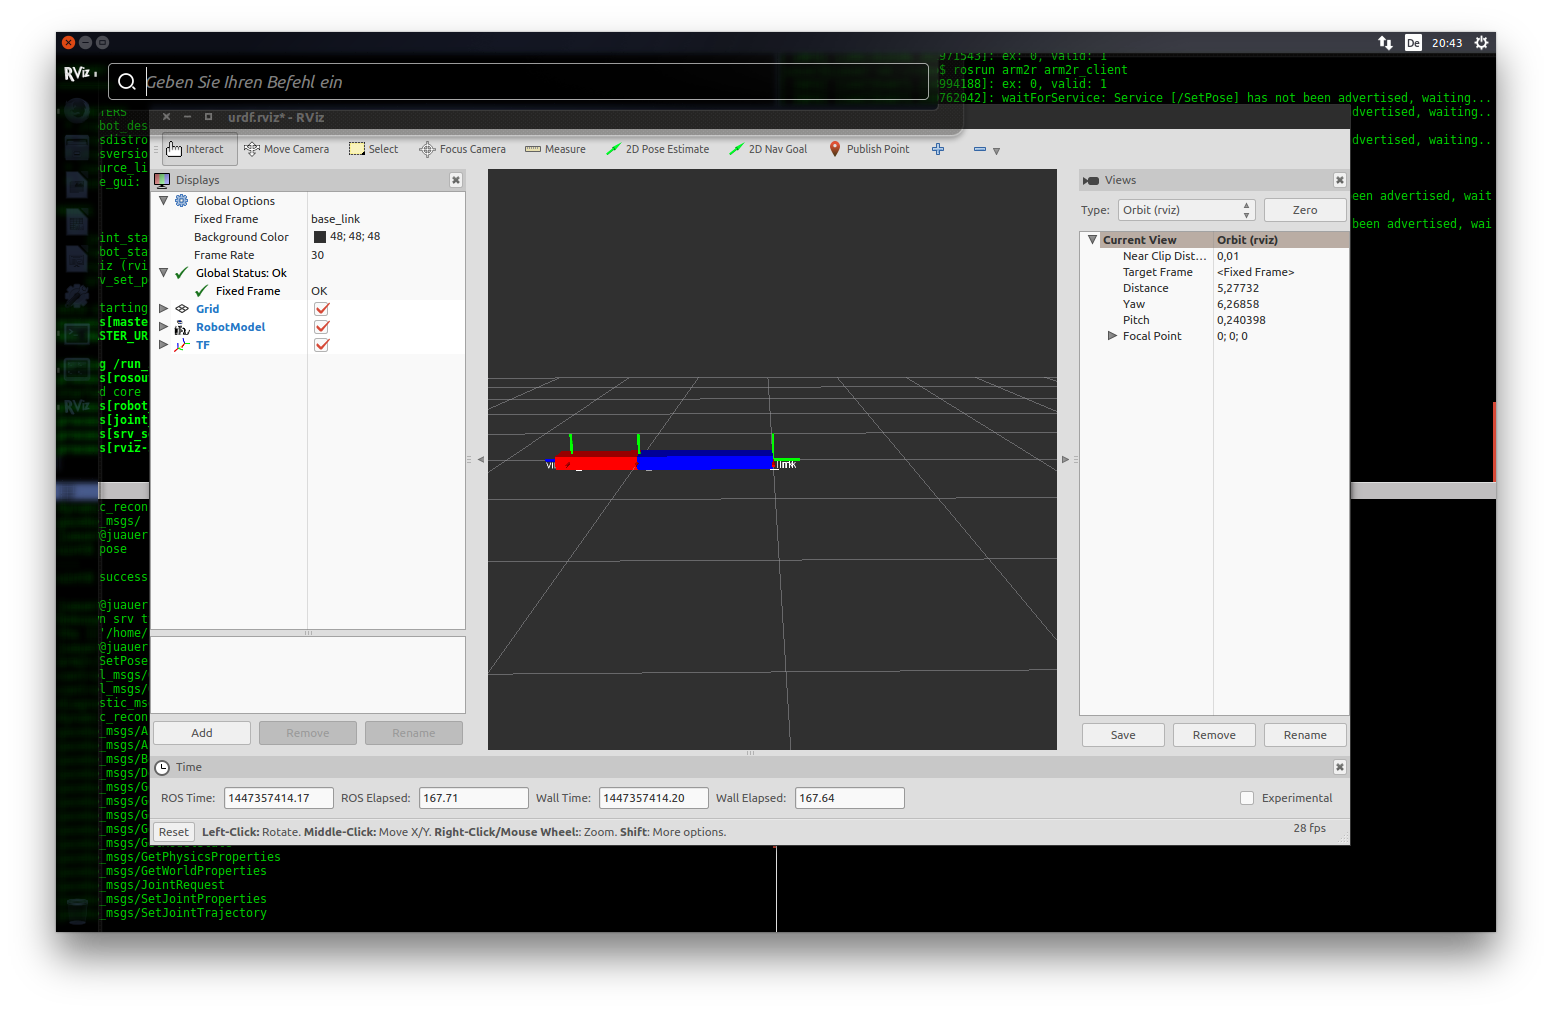
\includegraphics[width=0.8\linewidth]{capture_1-1}
}
\subfigure[nach oben]{
  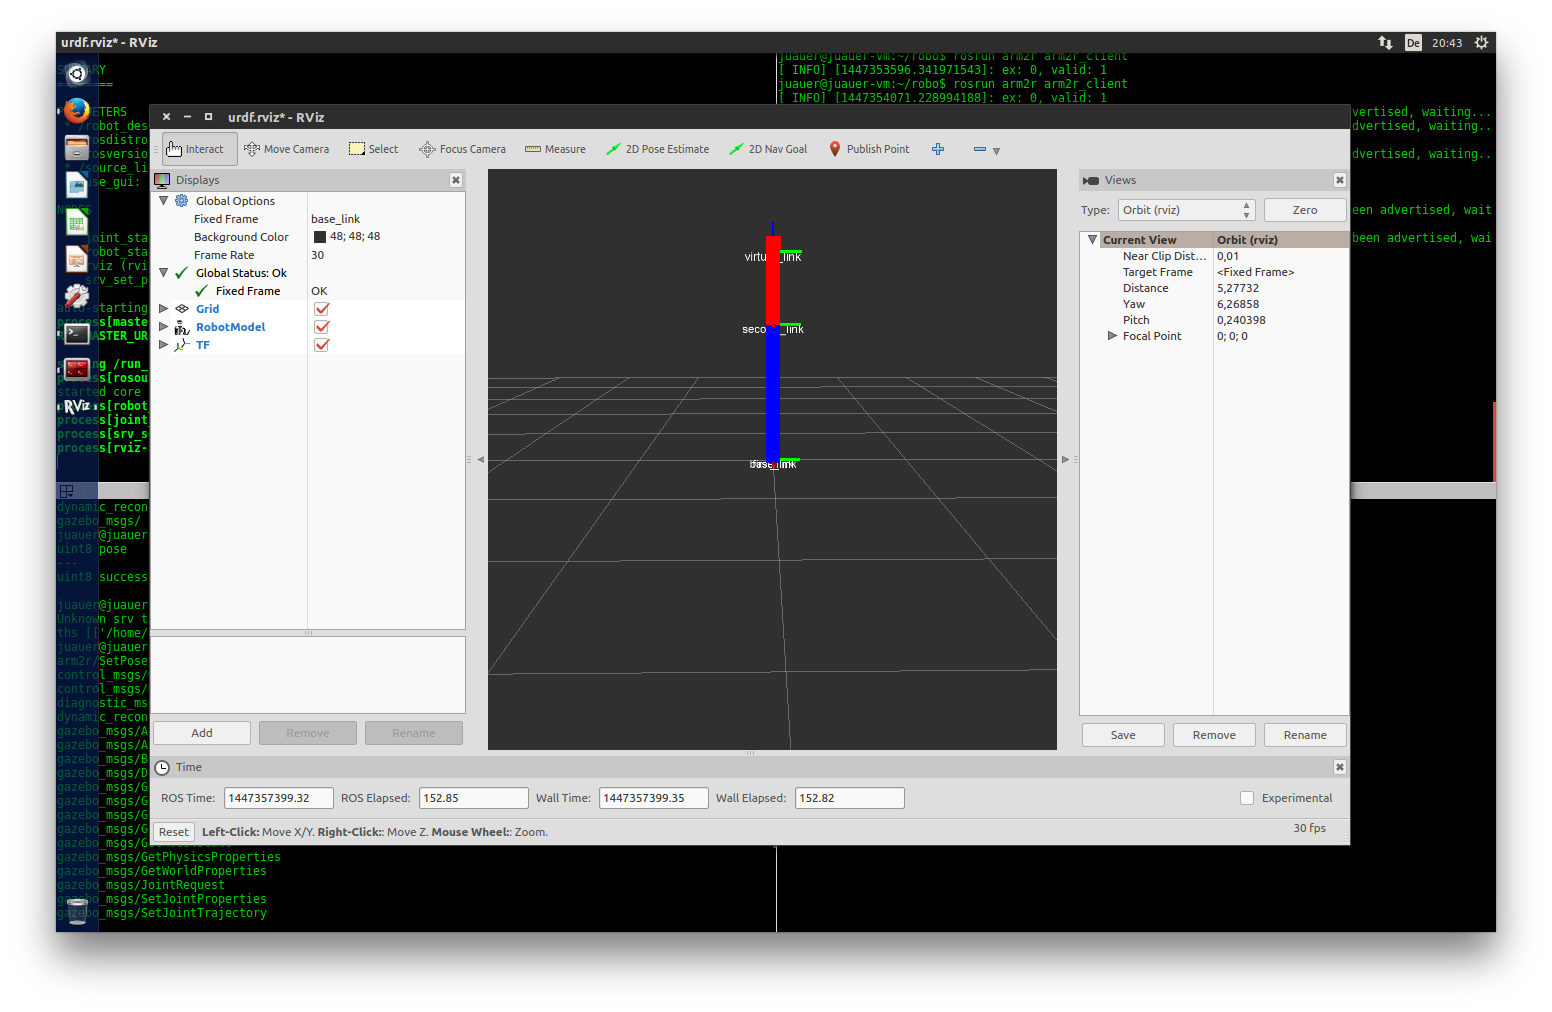
\includegraphics[width=0.8\linewidth]{capture_1-2}
}
\subfigure[nach rechts]{
  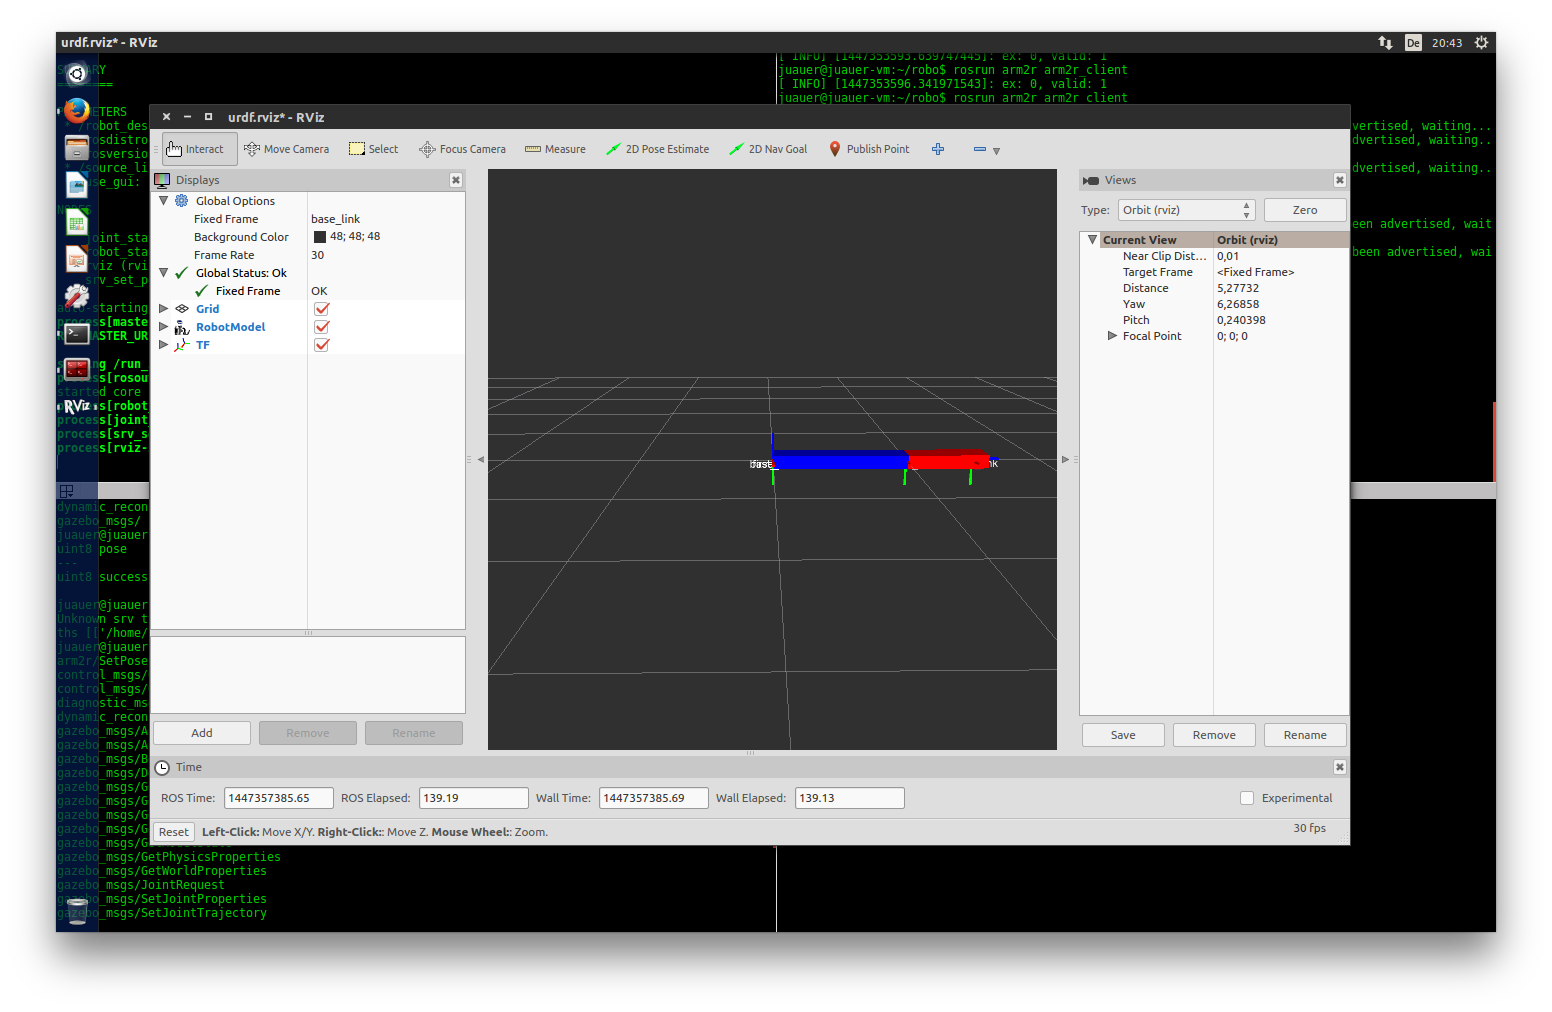
\includegraphics[width=0.8\linewidth]{capture_1-3}
}
\caption{Über Service getriggerte Bewegung}
\label{fig:1}
\end{figure}
\end{task}

\begin{task}{Roboter-Simulator Gezebo}
\item[]
Die Plugins zum Laufen zu bekommen, so dass sie mit dem vorbereiteten Code laufen war Horror. Ich habe stundenlang nur ''ruminstalliert''. Ganz fiese Aufgabe! Die normalen Gazebo-Tutorials liefen sofort problemlos - warum war es nötig, uns zusätzlich Code ''vorzubereiten'' der nur in einer sehr speziellen Software-Konfiguration läuft? Finde ich uncool.

\subtask{a}
Mit moveit habe ich keine Bewegung zustande bekommen: es ließ sich zwar etwas planen (siehe auch Abbildung \ref{fig:2-1}), Ineraktion mit den Gelenken war aber nicht möglich. Da es aber nirgendwo eine Fehlermeldung gab, hatte ich bei der ohnehin fiesen Aufgabe keine Lust, jetzt auch noch das Setup zu debuggen. Vielleicht Stoff für die Übung?

\begin{figure}[!htpb]
\centering
\subfigure[mit joint-trajectory-controller rqt-Plugin]{
  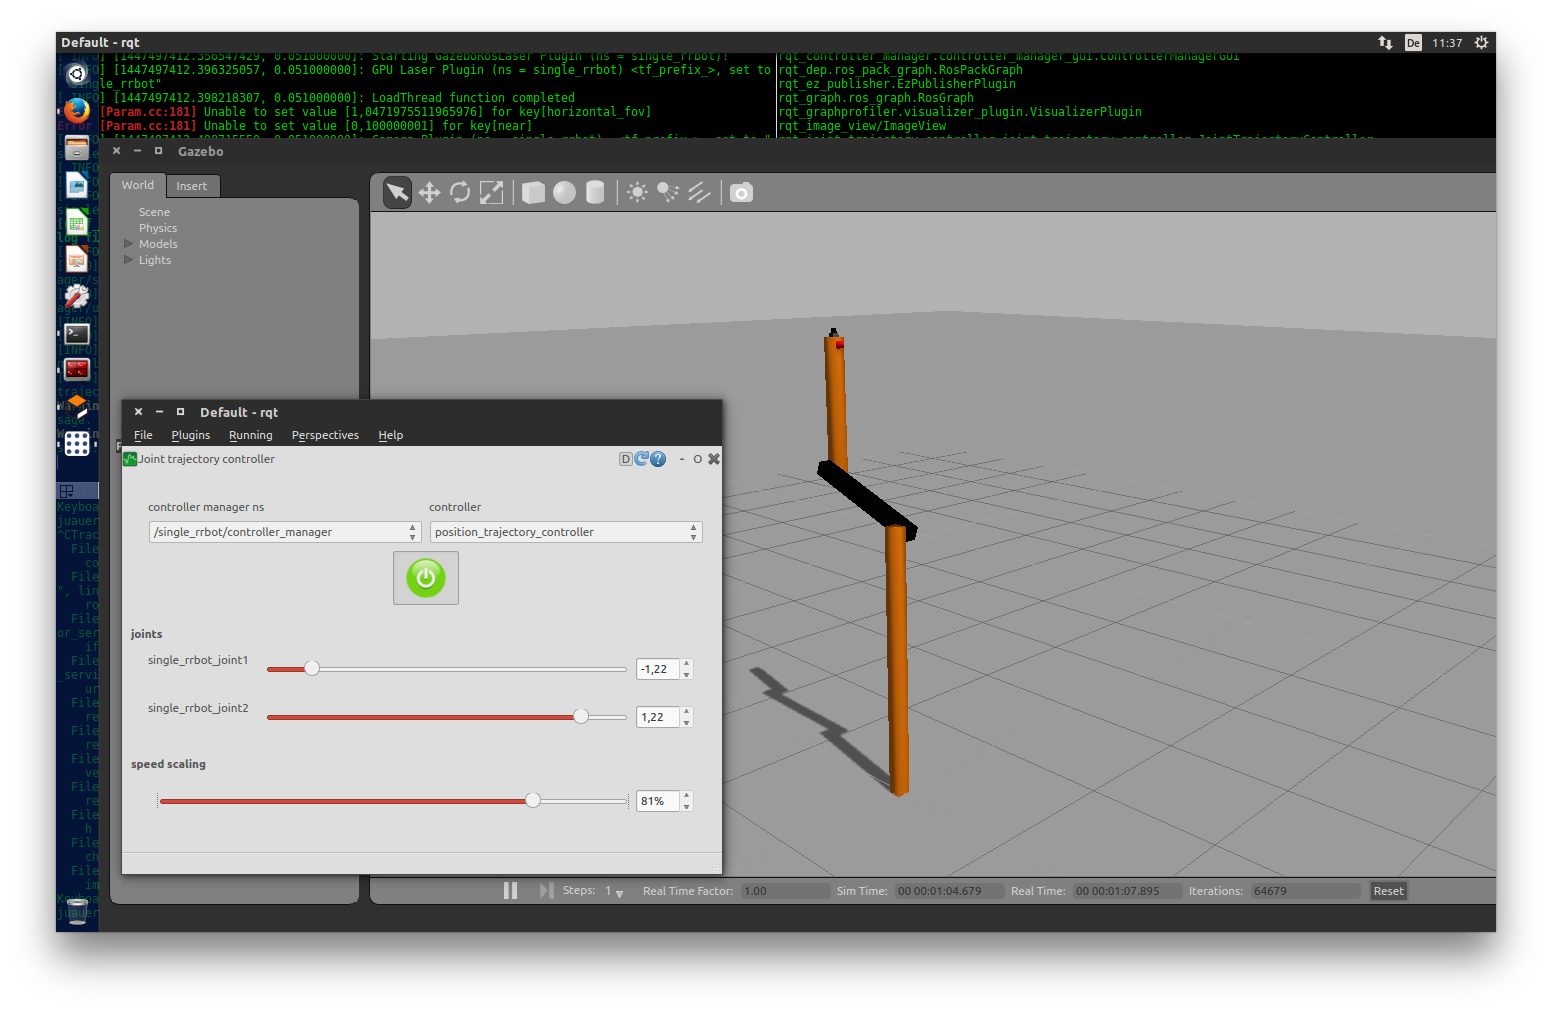
\includegraphics[width=0.8\linewidth]{capture_2-1}
}
\subfigure[mit moveit keine Joint-Interaktion möglich]{
  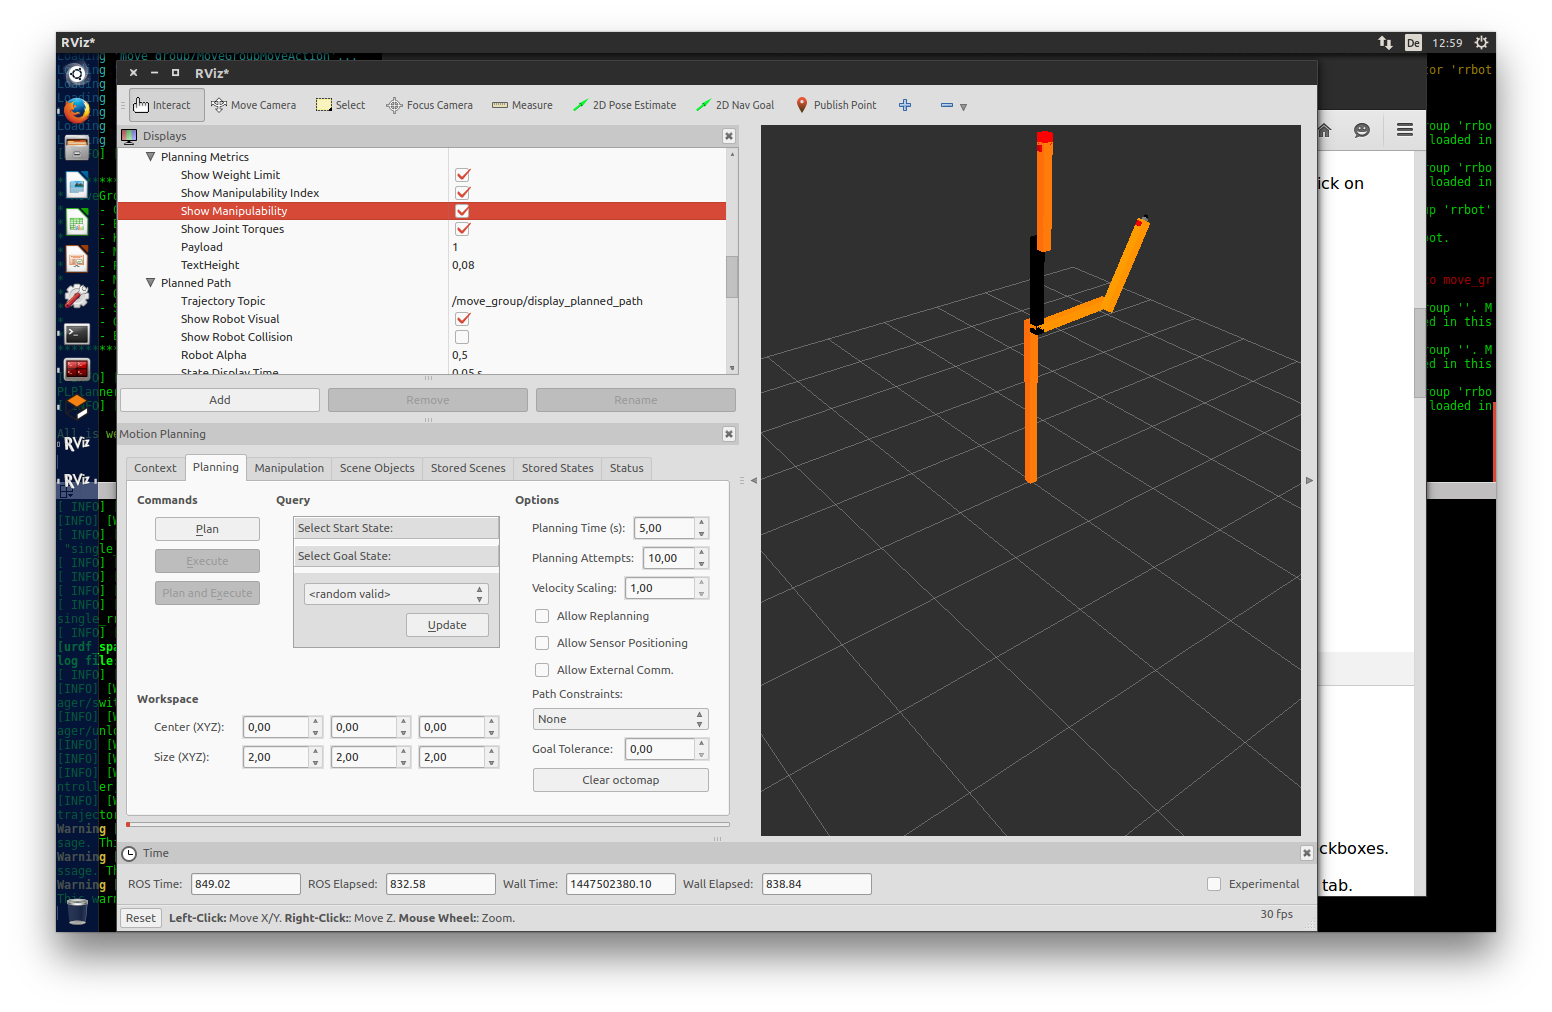
\includegraphics[width=0.8\linewidth]{capture_2-2}
}
\caption{Manuelle Steuerung \& Gazebo}
\label{fig:2-1}
\end{figure}

\subtask{b}
Siehe Code und Abbildung \ref{fig:2-2}.

\begin{figure}[!htpb]
\centering
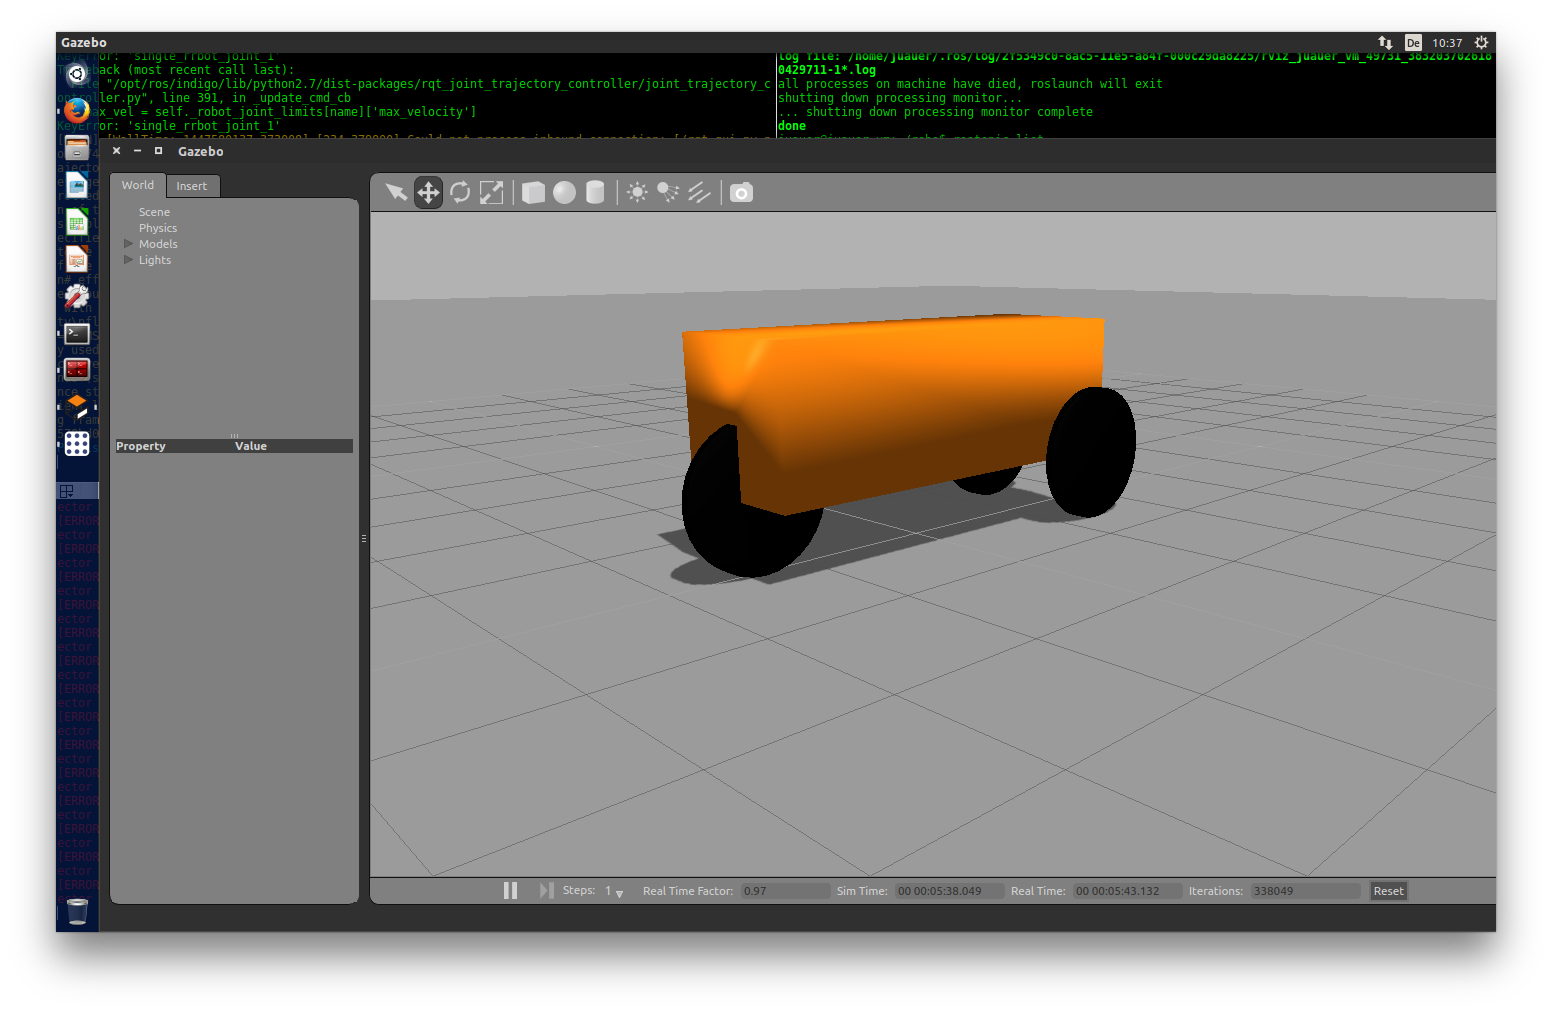
\includegraphics[width=0.8\linewidth]{capture_2-3}
\caption{Trike}
\label{fig:2-2}
\end{figure}
\end{task}

\begin{task}{Rotationen}
\subtask{a}
Auch bei Rotation um raumfeste Achsen spielt die Reihenfolge eine Rolle, zb. funktioniert hier
$$XYZ:(-90,0,-90)$$
wobei hingegen
$$ZYX:(-90,0,-90)$$
nicht funktioniert. Da keine Reihenfolge vorgegeben ist, lässt sich die Frage nicht eindeutig beantworten. Vielleicht ist ja auch ein Drehvektor gemeint?:
$$\sqrt{\frac{90^2}{2}}\cdot\begin{pmatrix}1\\-1\\0\end{pmatrix}$$
Mit einem Drehvektor würde man tatsächlich um nur eine raumfeste Achse rotieren.

\subtask{b}
$$ZYX:(-90,0,90)$$

\subtask{c}
$$ZYZ:(0,-90,-90)$$

\end{task}
\end{document}